\documentclass[12pt]{article}
\usepackage[english]{babel}
\usepackage[utf8x]{inputenc}
\usepackage[T1]{fontenc}
\usepackage{scribe}
\usepackage{wrapfig}
\usepackage{listings}
\usepackage{tikz}
\usepackage{comment}
\usepackage[demo]{float,graphicx}
\Scribe{Group 5 $\&$ Group 6}
\Lecturer{Abir De}
\LectureNumber{3}
\LectureDate{11 August 2022}
\LectureTitle{Linear Algebra Review, Classification Task}
\lstset{style=mystyle}

\begin{document}
	\MakeScribeTop

%#############################################################
%#############################################################
%#############################################################
%#############################################################

This lecture starts with a review of Linear Algebra and some of its usage in Machine Learning. Later on, the general ML problem of Classification is discussed.

\section{Linear Algebra (continued)}
Apart from the general usage of Linear Algebra in Machine Learning as a tool to represent features (as vectors/matrices) and weights (as matrices), there exist many tasks requiring deeper insights.

\subsection{Time Dependence in Networks}
Consider a classification task where we get sequences as input. In a normal classification task, features are of the form $\textbf{(\textit{feature}, \textit{label})}$ while for a sequence, there is a time component and each interval has a feature vector - $x_t, x_{t+1}, \dots$ with possible dependence across features. One possible relationship is a linear dependence of the features at time $t+1$ on the features at time $t$.

Suppose we have a network where edges represent influence of nodes over each other. This influence travels over time and the information/data at one node affects its neighbors and other nodes in the future. Social networks such as Facebook can be represented in this form and the information in the nodes can possibly be sentiment of people towards politicians or extent of spread of misinformation.

\begin{wrapfigure}{r}{0.3\textwidth}
  \begin{center}
    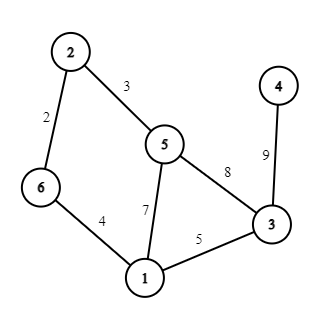
\includegraphics[width=0.28\textwidth]{graph.PNG}
  \end{center}
  \caption{Example Graph}
\end{wrapfigure}

Consider a graph similar to the one shown to the right. Suppose that nodes $i$ and $j$ share an influence over each other with strength $w_{ij} \text{ (not necessarily same as }w_{ji})$. For instance, the influence of $1$ over $6$ is twice that of $2$ over $6$ in the example graph (which is undirected, hence symmetric). These influences can be represented in a matrix $\mathbf{W}$ of size $N\times N$ where $N$ is the number of nodes in the graph. The elements on the diagonal $w_{ii}$  will represent remembrance of the previous state at some node.

Suppose the state at some time $t$ of the $i^{th}$ node is $\mathbf{x_t^i}$. These state vectors can be stacked row-wise in a matrix $\mathbf{X_t}$ which evolves with time. Assume that the state changes as following -
\[\mathbf{x_{t+1}^i} = {\sum_{j=1}^{n}w_{ij}\mathbf{x_{t}^j}}\]
Where n is the set of neighbours of node i\\
The evolution of states can then be represented as: $\mathbf{X_{t+1}} = \mathbf{W}\mathbf{X_t}$

\subsection{Stochastic Matrices}
Under some special conditions, the state denoted by $\mathbf{X_t}$ will converge. Such is the case of stochastic matrices.
\begin{definition}
Matrix $\mathbf{W}$ is \textbf{stochastic} if all entries are non-negative and sum of all entries in a column equals $1$. %$\mathbf{W}$ is further \textbf{positive} if all entries are positive numbers.
\end{definition}
\begin{lemma}Properties of eigenvalues of a stochastic matrix $\mathbf{W}$ are given below -
\begin{enumerate}
    \item $1$ is an eigenvalue of $\mathbf{W}$.
    \item If $\lambda$ is an eigenvalue (real/complex) of $\mathbf{W}$, $|\lambda|\leq1$.
\end{enumerate}
\end{lemma}
\noindent Some more important results related to stochastic matrices -
\begin{definition}
For a stochastic matrix $\mathbf{W}$, a \textit{steady state} is an eigenvector with eigenvalue $1$ whose entries are positive and add to $1$.
\end{definition}
\begin{theorem}[Perron-Frobenius Theorem]
For a positive stochastic matrix $\mathbf{W}$, there exists a unique steady state vector $v$ which spans the $1$-eigenspace. Also, for any vector $v_0$ with entries adding to $s$, iterates $v_1=Av_0, v_2=Av_1,\dots,v_{t+1}=Av_t,\dots$ tend to $sv$ as $t$ gets large.
\end{theorem}
\noindent More discussion can be found at \cite{interactivelinalg}.

\subsection{Average Consensus}
In this case, the weight matrix is such that all neighbors get equal weights and non-neighbors don't have any contribution. Suppose the graph is $G$ and its edge set is $E$.
\[\mathbf{x_{t+1}^i} = \frac{\sum_{j\in N(i)} \mathbf{x_{t}^j}}{|N(i)|}\]
Upon converting the equation to matrix form, we get the weight matrix $\mathbf{W}$ such that $w_{ij}=\frac{1}{d_i}$ (degree of vertex $i$) if $(i,j)\in E(G)$, else $w_{ij}=0$. Here, each sum rows to $1$ and this is a right stochastic matrix.

In this case, $\mathbf{1}$ is an eigenvector of $\mathbf{W}$ with eigenvalue $1$ because this multiplication just amounts to adding up every row which we already have as $1$.
\subsection{Non-convergence of state}
We can create instances of graphs where convergence is not reached. Consider the below graph with a central node \textbf{X} connected to some nodes (a star type network) . Suppose \textbf{X} has a state of $\mathbf{a}$ while all its neighbors have a value of $\mathbf{b}$. If the node state relation is a simple average over neighbors (average consensus), these values will keep oscillating - $\mathbf{a}$ on \textbf{X}, $\mathbf{b}$ on neighbors to $\mathbf{a}$ on neighbors, $\mathbf{b}$ on \textbf{X}. Convergence will never be reached in this case.




\tikzset{every picture/.style={line width=0.75pt}} %set default line width to 0.75pt        
\begin{center}
\begin{tikzpicture}[x=0.75pt,y=0.75pt,yscale=-1,xscale=1]
%uncomment if require: \path (0,470); %set diagram left start at 0, and has height of 470

%Shape: Circle [id:dp3817681879067485] 
\draw  [fill={rgb, 255:red, 0; green, 0; blue, 0 }  ,fill opacity=1 ] (160,149.67) .. controls (160,143.96) and (164.63,139.33) .. (170.33,139.33) .. controls (176.04,139.33) and (180.67,143.96) .. (180.67,149.67) .. controls (180.67,155.37) and (176.04,160) .. (170.33,160) .. controls (164.63,160) and (160,155.37) .. (160,149.67) -- cycle ;
%Shape: Circle [id:dp6935515903993525] 
\draw  [fill={rgb, 255:red, 0; green, 0; blue, 0 }  ,fill opacity=1 ] (231,219.67) .. controls (231,213.96) and (235.63,209.33) .. (241.33,209.33) .. controls (247.04,209.33) and (251.67,213.96) .. (251.67,219.67) .. controls (251.67,225.37) and (247.04,230) .. (241.33,230) .. controls (235.63,230) and (231,225.37) .. (231,219.67) -- cycle ;
%Shape: Circle [id:dp17989344932671902] 
\draw  [fill={rgb, 255:red, 0; green, 0; blue, 0 }  ,fill opacity=1 ] (156,61.67) .. controls (156,55.96) and (160.63,51.33) .. (166.33,51.33) .. controls (172.04,51.33) and (176.67,55.96) .. (176.67,61.67) .. controls (176.67,67.37) and (172.04,72) .. (166.33,72) .. controls (160.63,72) and (156,67.37) .. (156,61.67) -- cycle ;
%Shape: Circle [id:dp7221960494905768] 
\draw  [fill={rgb, 255:red, 0; green, 0; blue, 0 }  ,fill opacity=1 ] (74,214.67) .. controls (74,208.96) and (78.63,204.33) .. (84.33,204.33) .. controls (90.04,204.33) and (94.67,208.96) .. (94.67,214.67) .. controls (94.67,220.37) and (90.04,225) .. (84.33,225) .. controls (78.63,225) and (74,220.37) .. (74,214.67) -- cycle ;
%Straight Lines [id:da4291070055968442] 
\draw    (166.33,72) -- (170.33,139.33) ;
%Straight Lines [id:da725959440045093] 
\draw    (164,156) -- (90.33,208.33) ;
%Straight Lines [id:da13115299572109995] 
\draw    (236,210) -- (180.33,155.33) ;
%Shape: Circle [id:dp8297193155248772] 
\draw  [fill={rgb, 255:red, 0; green, 0; blue, 0 }  ,fill opacity=1 ] (426,153.67) .. controls (426,147.96) and (430.63,143.33) .. (436.33,143.33) .. controls (442.04,143.33) and (446.67,147.96) .. (446.67,153.67) .. controls (446.67,159.37) and (442.04,164) .. (436.33,164) .. controls (430.63,164) and (426,159.37) .. (426,153.67) -- cycle ;
%Shape: Circle [id:dp863785875888776] 
\draw  [fill={rgb, 255:red, 0; green, 0; blue, 0 }  ,fill opacity=1 ] (497,223.67) .. controls (497,217.96) and (501.63,213.33) .. (507.33,213.33) .. controls (513.04,213.33) and (517.67,217.96) .. (517.67,223.67) .. controls (517.67,229.37) and (513.04,234) .. (507.33,234) .. controls (501.63,234) and (497,229.37) .. (497,223.67) -- cycle ;
%Shape: Circle [id:dp37806146289546194] 
\draw  [fill={rgb, 255:red, 0; green, 0; blue, 0 }  ,fill opacity=1 ] (422,65.67) .. controls (422,59.96) and (426.63,55.33) .. (432.33,55.33) .. controls (438.04,55.33) and (442.67,59.96) .. (442.67,65.67) .. controls (442.67,71.37) and (438.04,76) .. (432.33,76) .. controls (426.63,76) and (422,71.37) .. (422,65.67) -- cycle ;
%Shape: Circle [id:dp0011330533956157574] 
\draw  [fill={rgb, 255:red, 0; green, 0; blue, 0 }  ,fill opacity=1 ] (340,218.67) .. controls (340,212.96) and (344.63,208.33) .. (350.33,208.33) .. controls (356.04,208.33) and (360.67,212.96) .. (360.67,218.67) .. controls (360.67,224.37) and (356.04,229) .. (350.33,229) .. controls (344.63,229) and (340,224.37) .. (340,218.67) -- cycle ;
%Straight Lines [id:da1910289900362534] 
\draw    (432.33,76) -- (436.33,143.33) ;
%Straight Lines [id:da6252849776059479] 
\draw    (430,160) -- (356.33,212.33) ;
%Straight Lines [id:da20183785416525213] 
\draw    (502,214) -- (446.33,159.33) ;
%Straight Lines [id:da4179412812743388] 
\draw    (250.33,119.67) -- (351,119.99) ;
\draw [shift={(353,120)}, rotate = 180.19] [color={rgb, 255:red, 0; green, 0; blue, 0 }  ][line width=0.75]    (10.93,-3.29) .. controls (6.95,-1.4) and (3.31,-0.3) .. (0,0) .. controls (3.31,0.3) and (6.95,1.4) .. (10.93,3.29)   ;

% Text Node
\draw (165,142) node [anchor=north west][inner sep=0.75pt]   [align=left] {\textcolor[rgb]{1,1,1}{a}};
% Text Node
\draw (236,212) node [anchor=north west][inner sep=0.75pt]   [align=left] {\textcolor[rgb]{1,1,1}{b}};
% Text Node
\draw (161,54) node [anchor=north west][inner sep=0.75pt]   [align=left] {\textcolor[rgb]{1,1,1}{b}};
% Text Node
\draw (79,207) node [anchor=north west][inner sep=0.75pt]   [align=left] {\textcolor[rgb]{1,1,1}{b}};
% Text Node
\draw (431,146) node [anchor=north west][inner sep=0.75pt]   [align=left] {\textcolor[rgb]{1,1,1}{b}};
% Text Node
\draw (502,216) node [anchor=north west][inner sep=0.75pt]   [align=left] {\textcolor[rgb]{1,1,1}{a}};
% Text Node
\draw (427,58) node [anchor=north west][inner sep=0.75pt]   [align=left] {\textcolor[rgb]{1,1,1}{a}};
% Text Node
\draw (345,211) node [anchor=north west][inner sep=0.75pt]   [align=left] {\textcolor[rgb]{1,1,1}{a}};
% Text Node
\draw (151,245) node [anchor=north west][inner sep=0.75pt]   [align=left] {Time \textbf{\textit{t}}};
% Text Node
\draw (402,243) node [anchor=north west][inner sep=0.75pt]   [align=left] {Time \textbf{\textit{t}}+1};
% Text Node
\draw (184,126) node [anchor=north west][inner sep=0.75pt]  [color={rgb, 255:red, 0; green, 0; blue, 0 }  ,opacity=1 ] [align=left] {X};
% Text Node
\draw (451,130) node [anchor=north west][inner sep=0.75pt]  [color={rgb, 255:red, 0; green, 0; blue, 0 }  ,opacity=1 ] [align=left] {X};


\end{tikzpicture}
\end{center}

\section{Introduction to the Classification Task}
Machine Learning deals with multiple tasks which can be broadly classified into Classification, Regression, Clustering etc. Of these, classification is a very important task. Consider the following Example,

We are given a set of images $\{I_1, \dots, I_n\}$, each corresponding to exactly one of three animal classes: cat, dog, or tiger. The pixel data of $I_i$ is encoded into feature-matrix $X_i \in \mathbb{R}^{d\times d}$, and IDs of the three classes are $\{0,1,2\}$ respectively. \textit{Binary} classification problems involve only two labels, usually $\{0,1\}$.
\\
\begin{figure}[H]

\centering
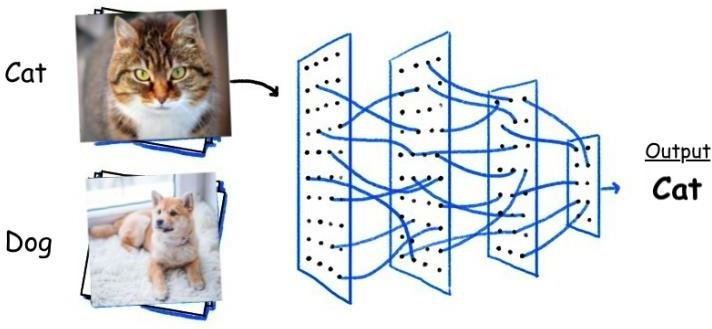
\includegraphics[scale=0.5]{classification.png}
\caption{Dog or Cat? A binary classification example }
\end{figure}
In General, we will be given $K$-dimensional input points, in the form of features  $X_1, X_2, \dots, X_K$,  our task will be to classify them into one of $N$ possible labels $1,2,\dots,N$.\\

\noindent\textbf{Solution Approach - }To solve the above task, we will need a function $\mathbf{H}$ such that $\mathbf{H}(X_i) = Y_i$ where $Y_i$ is the expected label for the input point with features $X_i$. The labels are defined by users, i.e., we don't know the definition or the meaning of a label. Suppose that no information about the relation between labels and features is provided to the function. A simple permutation of labels on the user side will lead to mistakes in the labels resulting from the function $\mathbf{H}$ even though the input didn't change. Hence, some information about the relation between labels and features is required. The easiest way to get this information is through examples, which is the first step in the solution method.
\begin{enumerate}
    \item Ask the user for information about labels in the form of examples i.e. $\{X_i, y_i\}_K$, formally known as \textbf{Training Set}.
\end{enumerate}
The user will provide us some already classified data (examples) and once we have the example pairs, the next step is to learn from them to be able to predict the labels for \textbf{unseen examples}.
\begin{enumerate}
    \item[2.] Create an algorithm \textbf{ALG} which \textit{learns} from provided examples and is able to do \textit{inference} i.e. predict labels for arbitrary input.
\end{enumerate}
Once the algorithm \textbf{ALG} is ready, we need to verify if it indeed works well for unseen inputs. For this, we would need some more examples as pairs to test results.
\begin{enumerate}
    \item[3.] Verify \textbf{ALG} on examples not included in the Training Set (checking the correctness of \textbf{ALG}). This set of examples is formally called the \textbf{Validation Set}. We don't use this set to edit the algorithm, it just helps accept/discard an algorithm.
\end{enumerate}
The entire  dataset is divided into the $2$ portions - \textbf{Training Set} \& \textbf{Validation Set}. Our goal during training is \textit{generalizability} - the algorithm should be as suitable for the Validation set as for the Training set. Relying only on training set performance isn't a good idea, since the model would have been overfitted on this data. Hence, After training the model (on the train set alone), its performance is evaluated on the validation set. Since the latter is unseen during training, we get more reliable estimate of the model's performance.

%%%%%%%%%%% If you don't have citations then comment the lines below:
%
\bibliographystyle{abbrv}           % if you need a bibliography
\bibliography{mybib}                % assuming yours is named mybib.bib

%%%%%%%%%%% end of doc
\end{document}